\documentclass[12pt]{article}

\usepackage{sbc-template}

\usepackage{graphicx,url}
\usepackage[utf8]{inputenc}
\usepackage[brazil]{babel}
\usepackage{amsmath}
\usepackage{booktabs}
\usepackage{hyperref}

\sloppy

\title{Previsão de Picos de Crimes Violentos e de Sinistros de Trânsito em
Dias de Jogos de Futebol na Cidade de São Paulo\\
\large Relatório Técnico Completo (sem limite de páginas)}

\author{Gilberto Serafim Dias de Araújo\inst{1}, Leonardo de Cico\inst{1},
Pedro Henrique de Almeida\inst{1}}

\address{Universidade de São Paulo (USP)\\
  São Paulo -- SP -- Brasil
  \email{serafimgilberto0@usp.br, leocico@usp.br, pedroalmeida04@usp.br}
}

\begin{document}

\maketitle

\begin{resumo}
Partidas de futebol concentram multidões em torno de estádios e alteram,
por algumas horas, as rotinas de deslocamento e convívio de uma cidade
inteira. Este trabalho construiu uma tabela analítica diária (730 dias,
2022--2023) integrando o calendário de partidas dos clubes de São Paulo
capital, registros oficiais de criminalidade e de sinistros de trânsito, e
variáveis de clima e calendário, e investigou empiricamente se dias de
jogo se associam a picos desses desfechos e se essa associação é
preditiva e/ou causal. Sete abordagens metodológicas independentes --
comparação ajustada por GLM Poisson, correlação parcial, modelo de
defasagens distribuídas, \emph{Difference-in-Differences} espacial,
\emph{Propensity Score Matching} com IPTW, uma adaptação de
\emph{Interrupted Time Series} e auditoria de colinearidade em valores de
SHAP -- convergem em um mesmo resultado: a associação bruta observada
desaparece após controle por calendário, e nenhum método encontra
evidência causal robusta de efeito do futebol. Um modelo XGBoost com
função de perda de Poisson superou os \emph{baselines} e o Prophet na
previsão da contagem diária de crimes violentos (MAE~34,8) e de sinistros
com vítima (MAE~10,3), validado por janela expansiva \emph{walk-forward};
uma Regressão Logística balanceada atingiu Recall de 0,58--0,67 na
identificação de dias de pico de sinistros com vítima, mas nenhum
classificador testado chegou a um ponto de operação útil para crimes
violentos. Este relatório documenta, sem restrição de espaço, todas as
etapas, métodos, números e decisões do projeto -- é a versão de
referência por trás do artigo curto no formato SBC.
\end{resumo}

\begin{abstract}
Football matches concentrate crowds around stadiums and disrupt, for a
few hours, the commuting and social routines of an entire city. This work
built a daily analytical table (730 days, 2022--2023) integrating the
match calendar of São Paulo football clubs, official records of criminal
occurrences and traffic accidents, and weather and calendar variables,
and empirically investigated whether game days are associated with peaks
in these outcomes, and whether that association is predictive and/or
causal. Seven independent methodological approaches converge on the same
result: the raw association disappears after controlling for calendar,
and no method finds robust causal evidence of a football effect. An
XGBoost model with a Poisson loss outperformed baselines and Prophet in
forecasting daily counts of violent crime (MAE~34.8) and injury traffic
accidents (MAE~10.3); a balanced Logistic Regression reached a Recall of
0.58--0.67 for injury-accident peak days, but no classifier reached a
useful operating point for violent crime. This report documents, without
space constraints, every stage, method, number and decision of the
project -- it is the full reference version behind the short SBC-format
paper.
\end{abstract}

\tableofcontents

\section{Introdução}

Grandes eventos esportivos são, do ponto de vista urbano, deslocamentos
temporários de rotina. Em poucas horas, dezenas de milhares de pessoas se
concentram no entorno de um estádio, alteram trajetos habituais, consomem
álcool em bares e praças de concentração e retornam simultaneamente para
casa ao final da partida. A Teoria da Atividade Rotineira \cite{cohen1979}
descreve exatamente esse cenário como propício à ocorrência de crimes: a
convergência, no tempo e no espaço, de ofensores motivados, alvos
disponíveis e ausência de vigilância capaz. São Paulo é um caso extremo
desse fenômeno no Brasil, por concentrar três clubes de série A que mandam
jogos na capital (Corinthians, Palmeiras e São Paulo FC -- o Santos manda
seus jogos em Santos-SP), quatro estádios de grande porte e uma agenda
que, entre campeonatos estadual, nacional, copas e competições
continentais, raramente deixa uma semana sem jogo na cidade. Ao mesmo
tempo, a disponibilidade de dados abertos sobre segurança pública,
sinistros de trânsito e clima tornou tecnicamente viável investigar essa
relação com métodos quantitativos, o que até pouco tempo dependia de
coleta manual e amostras pequenas.

O problema tratado neste trabalho é a investigação, em nível diário e
para o município de São Paulo, da associação entre a realização de
partidas de futebol e dias atípicos de violência e de sinistros de
trânsito, e da possibilidade de antecipar esses dias a partir do
calendário de jogos, das características de cada partida (mandante,
horário, clássico), das condições meteorológicas e do calendário civil. A
pergunta que orientou a investigação é concreta: conhecendo essas
variáveis com antecedência de um dia, é possível estimar se determinada
data apresentará volume de ocorrências acima do padrão -- e, indo além da
predição, existe evidência de que o jogo em si, e não o calendário que o
circunda, é responsável por essa eventual elevação? A delimitação da
unidade de análise foi deliberada: não se pretendeu localizar
espacialmente cada ocorrência; a unidade de análise é o dia na cidade, e
o produto é uma estimativa de risco potencialmente utilizável no
planejamento de efetivo policial e de fiscalização de trânsito.

Três dificuldades motivaram e ao mesmo tempo condicionaram esta
investigação. A primeira é metodológica: os trabalhos de referência sobre
o tema \cite{kurland2014,ristea2018,ristea2020} são espaciais e
explicativos, construídos sobre células de grade no entorno do estádio e
voltados a medir a associação entre evento e crime numa escala muito mais
fina do que a cidade inteira. A segunda é de disponibilidade de dados:
parte relevante do ganho preditivo relatado nesses estudos vem de
mensagens geolocalizadas de redes sociais, fonte cujo acesso programático
foi drasticamente restringido nos últimos anos, o que tornou necessário
verificar quanto sinal permanece recuperável apenas com dados oficiais e
de calendário. A terceira é a escassez de estudos que tratem crimes e
sinistros de trânsito como alvos de um mesmo pipeline: no contexto de
dias de jogo, ambos compartilham determinantes semelhantes --
aglomeração, consumo de álcool, deslocamento noturno concentrado --, mas
costumam ser estudados por comunidades separadas e sobre bases não
integradas.

O objetivo geral deste trabalho foi construir e avaliar um sistema de
ciência de dados que investigasse a associação entre o calendário de
jogos de futebol e picos de crimes violentos e de sinistros de trânsito
na cidade de São Paulo, e que estimasse esse risco em granularidade
diária. Foram perseguidos quatro objetivos específicos: (i) levantar e
integrar as fontes públicas necessárias, verificando a granularidade
efetivamente disponível em cada uma; (ii) especificar um pipeline de
integração que consolidasse fontes de granularidades distintas em uma
tabela analítica diária única; (iii) formular a tarefa preditiva, definir
um critério não arbitrário de pico e validá-lo temporalmente; e (iv) ir
além da predição, aplicando um conjunto de métodos de inferência causal
observacional para verificar se a associação encontrada, quando
existente, resiste ao controle por confundidores de calendário --
objetivo que extrapolou a ambição inicial do projeto e se tornou um dos
resultados centrais deste trabalho.

Este relatório é a versão completa, sem restrição de espaço, do artigo
submetido no formato SBC. Ele documenta cada etapa do pipeline com todos
os números, tabelas e decisões metodológicas -- inclusive as que foram
condensadas ou omitidas na versão curta por limite de página -- para
servir de referência técnica ao projeto e material de apoio à banca e aos
revisores.

\section{Trabalhos Relacionados}

A relação entre eventos esportivos e criminalidade urbana já foi estudada
sob perspectivas metodológicas distintas. Kurland et al.
\cite{kurland2014} examinaram o entorno do Villa Park (Aston Villa
Football Club, Birmingham) e mostraram que a distribuição espacial de
furtos e de crimes violentos contra a pessoa difere de forma significativa
entre dias de jogo e dias de comparação em um raio de aproximadamente três
quilômetros do estádio. O estudo é relevante aqui por dois motivos:
estabelece o desenho de dias de evento contra dias de controle
equivalentes, adotado nesta investigação, e evidencia que o efeito do
jogo, quando existe, não se restringe ao perímetro imediato do estádio --
o que motivou, aqui, testar tanto a escala de bairro quanto a escala da
cidade inteira.

Ristea et al. \cite{ristea2018} propuseram um dos primeiros arcabouços que
combinam dados criminais georreferenciados com mensagens do Twitter para
explicar a ocorrência de crimes ao redor de um estádio, agregando
ocorrências e mensagens geolocalizadas em células de 500\,m $\times$
500\,m e comparando oito horas em torno do início da partida em dias de
jogo e em dias de controle. Os autores mostraram que a densidade de
mensagens de conteúdo violento apresenta correlação espacial mais forte
com dano criminal, furto e violência contra a pessoa do que o volume total
de mensagens -- achado que sustenta um princípio adotado nesta
investigação: subconjuntos qualificados de um evento (aqui, clássicos e
jogos noturnos, e não simplesmente ``houve jogo'') podem ser mais
informativos do que o agregado indiferenciado, hipótese testada
explicitamente nos resultados.

Em trabalho posterior, Ristea et al. \cite{ristea2020} estenderam a
abordagem para Chicago, cruzando criminalidade, mensagens geolocalizadas
e variáveis demográficas, socioeconômicas e ambientais no entorno do
United Center, com estimação de densidade de kernel localizada e modelos
de previsão espacial para sete tipos de crime, comparando dias de jogo em
casa, jogos fora e dias de controle. A inclusão dos dados de redes
sociais elevou a AUC de previsão para quase todos os tipos de crime, com
ganhos maiores para furto de veículos e roubo e ganhos reduzidos para
crimes já fortemente concentrados no espaço e no tempo. Essa
heterogeneidade motivou, nesta investigação, a leitura desagregada por
grupo de atributos: era esperado que o efeito das variáveis de jogo fosse
desigual entre grupos de atributos, o que de fato ocorreu (Seção
\ref{sec:interpretabilidade}).

Os três trabalhos convergem em limitações que também condicionam esta
investigação: a defasagem e a granularidade heterogênea entre bases, e o
problema da unidade de área modificável (MAUP), pelo qual a escolha da
unidade espacial e temporal pode alterar substancialmente os resultados.
O posicionamento deste trabalho em relação a eles é triplo.
Metodologicamente, deslocou-se do objetivo espacial de fina granularidade
para um objetivo temporal e agregado à cidade inteira, adotando o dia em
São Paulo como unidade de análise. Quanto aos dados, substituiu-se a
fonte dinâmica de redes sociais -- indisponível em escala para o caso
brasileiro -- por atributos de partida conhecidos com antecedência, o que
tem a vantagem colateral de tornar o sistema utilizável de forma
prospectiva, e não apenas retrospectiva, tratando conjuntamente crimes e
sinistros de trânsito como alvos do mesmo pipeline. Por fim, ao contrário
dos trabalhos de referência, que têm objetivo primariamente
explicativo-espacial, este trabalho formalizou um bloco de inferência
causal observacional (pareamento por escore de propensão, ponderação por
probabilidade inversa de tratamento e uma adaptação de séries temporais
interrompidas), explicitando o quanto da associação observada resiste ao
controle por confundidores -- e não apenas relatando uma correlação
ajustada por regressão.

\section{Dados}
\label{sec:dados}

\subsection{Arquitetura bronze -- silver -- gold}

O pipeline de dados segue três camadas. A camada \emph{bronze} contém
cópias brutas de cada fonte, sem transformação. A camada \emph{silver}
contém uma tabela diária por fonte, já harmonizada e filtrada para o
município de São Paulo. A camada \emph{gold} contém os datasets
analíticos finais, usados diretamente pelas análises e modelos:
\texttt{fato\_dia\_sp.csv} (730 dias $\times$ 69 colunas, o dataset
analítico inicial), \texttt{pico\_dia\_sp.csv} (flags de pico, 730 dias
$\times$ 40 colunas) e \texttt{features\_dia\_sp.csv} -- o dataset final,
depois de toda a limpeza, definição de alvo e engenharia de atributos,
usado por todos os modelos preditivos (Seções \ref{sec:baselines} em
diante).

\subsection{O dataset final: \texttt{features\_dia\_sp.csv}}

\begin{table}[ht]
\centering
\caption{Visão geral do dataset final}
\small
\begin{tabular}{@{}ll@{}}
\toprule
Linhas & 730 (1 linha = 1 dia) \\
Período & 2022-01-01 a 2023-12-31 (contínuo) \\
Colunas & 109 \\
Chave primária & \texttt{data} \\
Unidade geográfica & Município de São Paulo (capital) \\
\bottomrule
\end{tabular}
\end{table}

As 109 colunas se organizam em cinco grupos:

\begin{itemize}
  \item \textbf{Temporais (26 colunas)}, todas conhecidas com
  antecedência: tendência linear, componentes cíclicas de dia do ano e
  dia da semana (\texttt{sin\_doy}/\texttt{cos\_doy},
  \texttt{sin\_dow}/\texttt{cos\_dow}), indicadores de dia da semana,
  mês, trimestre, semana do ano, fim de semana, feriado (nacional,
  estadual, municipal), véspera de feriado, período letivo, férias e
  recesso escolar;
  \item \textbf{Futebol (20 colunas)}: indicador de jogo, número de
  jogos, clássico, jogo noturno, defasagens $\pm1$/$\pm2$ dias do jogo e
  do clássico, jogos de Copa/Série A, número de jogos na janela de 7
  dias, dias desde/até o próximo jogo, interações jogo$\times$fim-de-
  semana e jogo$\times$noturno. Inclui também \texttt{publico} e
  \texttt{taxa\_ocupacao}, mantidas na tabela por transparência mas
  \textbf{100\% ausentes} -- a fonte (Kaggle,
  \texttt{adaoduque/campeonato-brasileiro-de-futebol}) nunca foi
  integrada;
  \item \textbf{Clima (11 colunas)}: temperatura média/máxima/mínima,
  precipitação total, umidade média, vento máximo, flag de chuva, flag
  de dado climático ausente, e as versões defasadas em 1 dia (variante
  conservadora que não assume previsão perfeita);
  \item \textbf{Históricas (38 colunas, 19 por alvo)}: para cada um dos
  2 desfechos principais, defasagens de 1, 2, 3, 7, 14, 28 e 364 dias,
  médias móveis e desvios-padrão móveis de 7, 14 e 28 dias, resíduo
  defasado, razão entre o valor defasado e a média móvel de 28 dias, e
  contagem de picos recentes. Toda feature histórica usa deslocamento
  $\geq 1$ dia, auditado automaticamente contra vazamento temporal (0
  falhas encontradas);
  \item \textbf{Alvos (10 colunas, 5 por desfecho)}: para
  \texttt{crimes\_violentos} e \texttt{acidentes\_com\_vitima} --
  contagem crua, resíduo dessazonalizado (o alvo de fato usado, Seção
  \ref{sec:definicao-pico}), pico no percentil 90 e 95 (booleano), e
  nível de risco em 3 categorias.
\end{itemize}

Quatro colunas adicionais registram o tratamento de qualidade aplicado:
\texttt{dia\_excluido\_crime} (3 dias excluídos: censura de fim de série e
lacuna de registro Infosiga), \texttt{dia\_excluido\_acidente} (4 dias) e
\texttt{dia\_artefato\_lote} (1 dia -- o pico de furtos em lote de
19/06/2022).

\begin{table}[ht]
\centering
\caption{Estatísticas descritivas dos 2 alvos principais (contagem diária)}
\small
\begin{tabular}{@{}lrrrrr@{}}
\toprule
\textbf{Alvo} & \textbf{$n$ válido} & \textbf{Média} & \textbf{DP} & \textbf{Mín.} & \textbf{Máx.} \\
\midrule
Crimes violentos     & 727 & 517,7 & 65,4 & 340 & 755 \\
Sinistros com vítima & 726 & 80,9  & 15,5 & 31  & 125 \\
\bottomrule
\end{tabular}
\end{table}

Nenhum dos dois alvos tem contagem zero em nenhum dia do período, o que
torna o MAPE (erro percentual absoluto médio) uma métrica estável e
interpretável -- e o SMAPE, cuja principal vantagem é lidar com valores
próximos de zero, desnecessário neste caso.

\section{Metodologia}

A metodologia está organizada em dois blocos, seguindo a lógica adotada
por Soliani et al. \cite{soliani2024} ao investigar acidentes com
caminhões em rodovias brasileiras: um bloco explicativo, que estabelece
se e como o calendário de jogos se associa aos desfechos de interesse, e
um bloco preditivo, que usa essa base para construir e validar modelos de
previsão de picos. A Figura~\ref{fig:pipeline} resume as quatro etapas do
pipeline -- integração de dados, análise exploratória e causal, definição
do alvo e engenharia de atributos, e modelagem preditiva --, no espírito
do diagrama de estágios de da Silva et al. \cite{dasilva2025}.

\begin{figure}[ht]
\centering
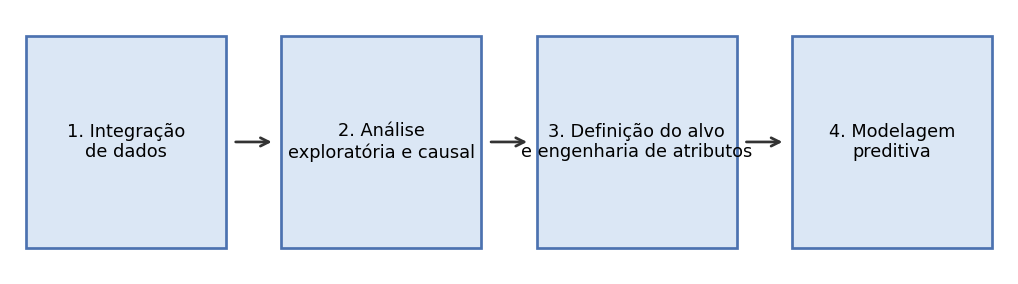
\includegraphics[width=.95\linewidth]{figuras/pipeline.png}
\caption{Etapas do pipeline de dados e análise}
\label{fig:pipeline}
\end{figure}

\subsection{Fontes de dados e integração}

Quatro categorias de dados públicos foram integradas para o município de
São Paulo, no período de 2022-01-01 a 2023-12-31 (730 dias, a janela de
sobreposição entre as três fontes principais):

\begin{itemize}
  \item \textbf{Criminalidade}: SPDadosCriminais (SSP-SP), microdados de
  boletim de ocorrência, filtrados por código IBGE do município
  (3550308) -- o campo textual da cidade apresenta variações de
  formatação que o tornam pouco confiável como filtro isolado. O grão
  real da fonte é boletim $\times$ rubrica, não boletim único;
  \item \textbf{Sinistros de trânsito}: Infosiga SP (Detran-SP), mesmo
  filtro geográfico, granularidade de evento, encoding latin-1;
  \item \textbf{Partidas de futebol}: base histórica de jogos do
  Campeonato Brasileiro (Séries A/B/C) e Copa do Brasil, restrita aos
  mandantes que jogam na capital (Corinthians, Palmeiras e São Paulo FC
  -- o Santos manda seus jogos em Santos-SP, fora do escopo geográfico).
  Campeonato Paulista e Libertadores não estão cobertos por esta base;
  \item \textbf{Clima e calendário}: estação meteorológica INMET A701
  (São Paulo -- Mirante), agregada de horária para diária (fuso
  UTC$\to$Brasília, $-3$h fixo); feriados nacionais, estaduais e
  municipais calculados algoritmicamente; calendário escolar da rede
  municipal transcrito manualmente das resoluções oficiais.
\end{itemize}

Cada fonte foi agregada ao grão \emph{dia} e unida por uma chave de
calendário mestre, garantindo que dias sem jogo, sem chuva ou sem
ocorrência apareçam com valor zero explícito, não como linha ausente.

Dois cuidados de qualidade merecem registro, por afetarem diretamente a
validade das análises subsequentes. Primeiro, os últimos dois dias da
série (30 e 31 de dezembro de 2023) apresentam contagens de criminalidade
e sinistros anormalmente baixas -- um efeito de defasagem no registro
administrativo dos boletins, não uma queda real de ocorrências -- e foram
excluídos de todas as análises de teste de hipótese e de treinamento.
Segundo, um dia isolado (19 de junho de 2022) apresenta um pico isolado
de furtos ($\texttt{furtos\_total}=2633$ vs.\ mediana $\sim$780)
compatível com lançamento retroativo em lote pela fonte primária; seu
tratamento foi avaliado por análise de sensibilidade (Seção
\ref{sec:validacao}) e, na engenharia de atributos, as contagens de crime
desse dia foram marcadas como ausentes (não removidas nem zeradas), com
os lags interpolando apenas o buraco de um dia. Outras lacunas
documentadas: 2022-01-17 e 2023-08-07 (falha do fluxo de notificação da
Infosiga), 27/11/2023 (falha total do INMET) e 25/08 a 11/09/2023
(sensor de precipitação fora do ar).

\subsection{Bloco explicativo: associação entre jogos e desfechos}

Antes de qualquer modelo preditivo, testou-se se dias de jogo se associam
a desfechos elevados de criminalidade e sinistros, e se essa associação
sobrevive ao controle por fatores de calendário -- réplica do cuidado de
Soliani et al. \cite{soliani2024} em separar a análise de causas da etapa
de predição por aprendizado de máquina.

\textbf{Comparação bruta e ajustada.} Dias com e sem jogo foram
comparados por teste de Mann--Whitney (dados de contagem, distribuição
não-normal confirmada por teste de normalidade prévio), com correção de
Benjamini--Hochberg \cite{bh1995} para múltiplas comparações. Em seguida,
a associação foi reestimada por Modelo Linear Generalizado com
distribuição de Poisson e erros-padrão robustos (HC1),
\begin{equation}
\log(\mathrm{E}[y_d]) = \beta_0 + \beta_1\,\text{jogo}_d +
  \gamma\,\text{diaSemana}_d + \delta\,\text{mês}_d + \epsilon\,\text{feriado}_d,
\end{equation}
controlando explicitamente por dia da semana e mês -- este último
necessário porque a temporada de futebol (abril--novembro) não cobre o
verão (dezembro--março), o que poderia confundir efeito de jogo com
efeito sazonal. Como robustez adicional, um segundo modelo de controle
acrescentou temperatura, precipitação e umidade (subamostra
$n\approx713$, dias com clima observado).

\textbf{Defasagem temporal.} Um modelo de defasagens distribuídas
($\text{jogo}_{d-2}\ldots\text{jogo}_{d+2}$) avaliou se o efeito, caso
exista, precede ou sucede o dia do jogo. Uma correlação cruzada sobre
séries dessazonalizadas (resíduo de
$\text{OLS}(y \sim \text{diaSemana} + \text{mês} + \text{feriado})$) e um
\emph{event study} (média do resíduo em offsets $-7$ a $+7$ dias em
torno de cada jogo, para todos os jogos e para jogos isolados) serviram
como checagens exploratórias complementares.

\textbf{Análise espacial.} Para o crime, cuja coordenada bruta tem
$\sim$20\% de valores nulos, zero ou externos ao município, o bairro foi
adotado como unidade primária; o anel de distância ($\leq2,5$\,km vs.\
7,5--15\,km do estádio) serviu como robustez secundária. Um
\emph{Difference-in-Differences} testou a interação
estádio-bairro$\times$jogo, com e sem as duas datas de maior público da
base.

\textbf{Causalidade formal.} Cobrindo os métodos indicados na literatura
de inferência causal com dados observacionais, aplicou-se pareamento por
escore de propensão (\emph{Propensity Score Matching}, vizinho mais
próximo, \emph{caliper} de 0,2 desvio-padrão do logit do escore, seguindo
Austin \cite{austin2011}) e ponderação por probabilidade inversa de
tratamento (IPTW) como robustez, além de uma adaptação de
\emph{Interrupted Time Series} em torno do evento de maior público da
base. A violação de positividade (ausência de dias de jogo em
janeiro--fevereiro) foi verificada explicitamente antes do pareamento,
seguindo a prática recomendada de checar sobreposição de suporte antes de
interpretar qualquer estimativa de efeito causal.

\subsection{Definição da variável-alvo}
\label{sec:definicao-pico}

Em vez de um limiar arbitrário sobre a contagem bruta -- que se mostrou
equivalente, na prática, a um classificador de fim de semana (25\% das
sextas-feiras seriam ``pico'' contra 1\% das segundas, usando a contagem
crua) --, o alvo de ``pico'' foi definido sobre o resíduo dessazonalizado:
um dia é considerado pico quando esse resíduo excede o percentil 90 da
sua distribuição histórica. Percentil 90 foi escolhido como método
principal (produz $\sim$10\% de dias-pico, base suficiente para
validação); z-score e média móvel causal de 28 dias foram mantidos como
variantes de robustez. O nível de risco em 3 categorias (Baixo/Médio/Alto
= $<$P75/P75--P90/$>$P90 do resíduo) usa exclusivamente o resíduo de
crimes violentos, sem combinar os dois domínios num índice único.

\subsection{Bloco preditivo: engenharia de atributos e modelos}
\label{sec:baselines}

\textbf{Atributos.} Quatro grupos de variáveis foram construídos:
temporais (calendário, sazonalidade), de futebol (mandante, clássico,
horário, restritas a informação disponível com antecedência -- resultado
e gols do próprio jogo foram excluídos por vazamento de informação),
climáticas, e históricas (defasagens de 1 a 28 e 364 dias e médias
móveis do próprio desfecho, sempre com deslocamento mínimo de 1 dia para
impedir vazamento temporal). Ver detalhamento completo na Seção
\ref{sec:dados}.

\textbf{Baselines.} Para regressão: média histórica, média móvel (7 e 28
dias) e mesmo dia da semana anterior. Para classificação: classe
majoritária e uma heurística de calendário (\texttt{dia\_semana\_risco},
dias da semana com taxa de pico acima da média no treino).

\textbf{Modelos e validação.} Seguindo o mesmo cuidado de comparação
contra baseline adotado por Soliani et al. \cite{soliani2024} (que
compararam oito classificadores contra referências simples antes de
escolher o melhor), testaram-se os baselines contra Decision Tree, Random
Forest, HistGradientBoosting, XGBoost \cite{chen2016} e LightGBM
(regressão com função de perda de Poisson, adequada a dados de contagem)
e Regressão Logística (classificação, com e sem balanceamento de classe).
A validação usou janela expansiva com 12 \emph{folds} mensais
(\emph{walk-forward}), ancorada em 2022-01-01 e cobrindo 2023 inteiro em
teste, nunca divisão aleatória -- dado que a ordem temporal é informativa
e uma divisão aleatória permitiria que o modelo ``veja o futuro'' durante
o treino. Em cada \emph{fold}, o limiar de pico e o ajuste de calendário
foram reestimados exclusivamente sobre os dados de treino daquele
\emph{fold}, para impedir vazamento de informação do teste. O Prophet
\cite{taylor2018} (sobre $\log(1+y)$) foi comparado ao XGBoost nos mesmos
\emph{folds}, sendo esta a comparação central do título do projeto.

\textbf{Métricas.} Regressão: MAE, RMSE, $R^2$, MAPE (SMAPE avaliado como
desnecessário, Seção \ref{sec:dados}). Classificação: Acurácia,
Precisão, Recall, $F_1$, ROC-AUC e PR-AUC -- nunca escolhendo o modelo
apenas pela acurácia. Métricas agregadas tanto \emph{pooled} (previsões
de todos os \emph{folds} empilhadas) quanto \texttt{fold\_macro} (métrica
calculada dentro de cada \emph{fold}, depois com média entre
\emph{folds}) -- a segunda é mais robusta quando há poucos positivos por
\emph{fold} (Seção \ref{sec:validacao}).

\textbf{Otimização de hiperparâmetros.} Realizada por busca aleatória
aninhada (\emph{nested walk-forward}): o nível externo replica os mesmos
12 \emph{folds} da validação (métrica pooled comparável), o nível interno
usa \texttt{TimeSeriesSplit} dentro do treino de cada \emph{fold}
externo -- de modo que a escolha de hiperparâmetros para o mês de teste
do \emph{fold} $n$ nunca observa dados do \emph{fold} $n$ ou posteriores.
Hiperparâmetros de \emph{produção} (usados nos modelos finais explicados
por SHAP) vieram de uma busca separada sobre todo o histórico, fora da
métrica de validação reportada.

\textbf{Interpretabilidade.} A contribuição de cada grupo de atributos
foi quantificada por valores de Shapley (SHAP) \cite{lundberg2017}, com
\texttt{TreeExplainer} para os modelos de árvore e explicador linear para
a regressão logística. Atributos com contribuição elevada foram
auditados quanto à colinearidade com variáveis de calendário antes de
serem atribuídos a um efeito de futebol -- um cuidado necessário porque
atributos de contagem de dias até o próximo jogo mostraram-se, no caso
deste estudo, proxies quase perfeitos de época do ano.

\textbf{Cenários.} Simulações de cenário (domingo com jogo comum, domingo
com clássico, quarta-feira com jogo noturno, domingo com clássico sob
chuva) foram construídas a partir de dias reais do conjunto de dados que
satisfazem cada descrição -- não de vetores de atributos sintéticos --,
evitando fabricar combinações de variáveis sem respaldo empírico. A
diferença entre cada cenário e seu par de referência foi decomposta por
grupo de atributos via aditividade dos valores SHAP, na escala em que o
modelo é aditivo (log da taxa para o XGBoost Poisson, log-odds para a
Regressão Logística).

\section{Resultados}

\subsection{Associação bruta e ajustada entre jogo e desfechos}

A comparação bruta entre dias com e sem jogo (teste de Mann--Whitney,
correção de Benjamini--Hochberg para 11 desfechos) mostrou diferenças
estatisticamente significativas para vários desfechos, resumidas na
Tabela~\ref{tab:bruto}.

\begin{table}[ht]
\centering
\caption{Comparação bruta dia-com-jogo vs.\ dia-sem-jogo (Mann--Whitney,
correção BH)}
\label{tab:bruto}
\small
\begin{tabular}{@{}lrrl@{}}
\toprule
\textbf{Desfecho} & \textbf{Dif.\ (\%)} & \textbf{$p$ (BH)} & \textbf{Signif.\ 5\%} \\
\midrule
Crimes violentos          & $-0,1$  & $0,775$  & Não \\
Roubos totais             & $-3,3$  & $0,032$  & Sim \\
Lesão corporal dolosa     & $+14,9$ & $<0,001$ & Sim \\
Sinistros totais          & $+6,3$  & $0,001$  & Sim \\
Sinistros com vítima      & $+4,6$  & $0,032$  & Sim \\
Sinistros fatais          & $+38,7$ & $<0,001$ & Sim \\
\bottomrule
\end{tabular}
\end{table}

Nenhuma dessas diferenças, porém, sobreviveu ao ajuste por GLM Poisson
com erros HC1 controlando dia da semana, mês e feriado
(Tabela~\ref{tab:glm}): todas as razões de taxas (RR) ajustadas ficaram
estatisticamente indistinguíveis de 1 após correção de múltiplas
comparações. O resíduo mais próximo de significância em todo o projeto
foi sinistros fatais, $\text{RR}=1,146$ ($\text{IC}_{95\%}\,
0,993$--$1,323$, $p=0,063$ sem correção, $p_{BH}=0,575$).

\begin{table}[ht]
\centering
\caption{Associação ajustada entre dia de jogo e desfechos (GLM Poisson,
erros HC1, controlando dia da semana, mês e feriado)}
\label{tab:glm}
\small
\begin{tabular}{@{}lrrrr@{}}
\toprule
\textbf{Desfecho} & \textbf{RR} & \textbf{IC 95\%} & \textbf{$p$} & \textbf{$p_{BH}$} \\
\midrule
Crimes totais           & $1,020$ & $0,990$--$1,050$ & $0,197$ & $0,575$ \\
Crimes violentos        & $1,009$ & $0,988$--$1,031$ & $0,399$ & $0,575$ \\
Roubos totais           & $1,009$ & $0,984$--$1,035$ & $0,471$ & $0,575$ \\
Furtos totais           & $1,025$ & $0,983$--$1,068$ & $0,249$ & $0,575$ \\
Lesão corporal dolosa   & $1,015$ & $0,975$--$1,057$ & $0,462$ & $0,575$ \\
Homicídios dolosos      & $0,907$ & $0,758$--$1,085$ & $0,286$ & $0,575$ \\
Sinistros totais        & $1,002$ & $0,972$--$1,033$ & $0,902$ & $0,902$ \\
Sinistros com vítima    & $1,015$ & $0,985$--$1,046$ & $0,333$ & $0,575$ \\
Atropelamentos          & $1,035$ & $0,968$--$1,106$ & $0,315$ & $0,575$ \\
Colisões                & $1,010$ & $0,976$--$1,046$ & $0,556$ & $0,612$ \\
Sinistros fatais        & $1,146$ & $0,993$--$1,323$ & $0,063$ & $0,575$ \\
\bottomrule
\end{tabular}
\end{table}

A correlação parcial de Spearman entre 4 indicadores de jogo
(ocorrência, número de jogos, clássico, jogo noturno) e os 11 desfechos,
controlando os mesmos confundidores, não encontrou nenhum dos 44 pares
significativo após Benjamini--Hochberg em nenhum dos dois modelos de
controle (A: calendário; B: calendário + clima, $n\approx713$) --
contra 8 dos 44 pares significativos na correlação de ordem zero (sem
controle). Um modelo de defasagens distribuídas
($\text{jogo}_{d-2}\ldots\text{jogo}_{d+2}$, 6 desfechos $\times$ 5
defasagens = 30 estimativas) não encontrou nenhuma defasagem
significativa após correção; o \emph{event study} em torno de cada jogo
(offsets $-7$ a $+7$ dias) também não encontrou desvio significativo em
nenhum offset, para jogos isolados ou para todos os jogos.

\subsection{Análise espacial}

Na escala de bairro, o \emph{Difference-in-Differences} em torno dos 3
principais estádios encontrou razão de taxas aparente de $2,39$
($\text{IC}_{95\%}\,1,13$--$5,05$, $p=0,023$, $p_{BH}=0,068$ ns) para o
bairro do Estádio do Morumbi, contra $1,01$ (Allianz Parque) e $0,91$
(Neo Química Arena, ambos ns). A razão do Morumbi caiu para $1,17$
($p=0,136$ ns) ao remover apenas duas datas -- a final e a semifinal da
Copa do Brasil 2023, os dois jogos de maior público de toda a base. A
investigação subsequente mostrou três mecanismos concretos por trás desse
RR aparente: (i) concentração nessas 2 datas específicas, não em dia de
jogo comum; (ii) $\sim$60\% dos registros geocodificados nas mesmas duas
coordenadas do próprio estádio -- um artefato do sistema de
geocodificação de boletins de ocorrência \emph{online} (endereço
declarado, não local real); e (iii) $75\%+$ dos casos são furto simples,
não crime violento.

Como robustez secundária (a coordenada bruta de crime tem $\sim$20\% de
valores inválidos), um DiD por anel de distância ($\leq2,5$\,km vs.\
7,5--15\,km) foi testado com e sem as 2 datas de alavancagem
(Tabela~\ref{tab:did-anel}). O Morumbi confirma o mesmo padrão (RR cai de
$2,66$ para $1,24$, $p=0,078$, ns, ao remover as 2 datas); a Allianz
Parque mostra um RR de crime persistentemente $\sim$$1,17$--$1,18$
($p\approx0,02$--$0,03$), mas sem \emph{pile-up} de coordenada e sem
aparecer na análise de bairro -- tratado como ruído do método por anel,
não como achado.

\begin{table}[ht]
\centering
\caption{DiD por anel de distância (crime), com e sem as 2 datas de
alavancagem}
\label{tab:did-anel}
\small
\begin{tabular}{@{}llrr@{}}
\toprule
\textbf{Estádio} & \textbf{Amostra} & \textbf{RR} & \textbf{$p$} \\
\midrule
Neo Química Arena  & Todos os jogos   & $0,954$ & $0,369$ \\
Neo Química Arena  & Sem 2 datas      & $0,955$ & $0,374$ \\
Allianz Parque     & Todos os jogos   & $1,175$ & $0,022$ \\
Allianz Parque     & Sem 2 datas      & $1,170$ & $0,026$ \\
Estádio do Morumbi & Todos os jogos   & $2,661$ & $0,016$ \\
Estádio do Morumbi & Sem 2 datas      & $1,238$ & $0,078$ \\
\bottomrule
\end{tabular}
\end{table}

\textbf{Achado colateral (Fisher exato).} Dos 12 dias-pico de consenso
(percentil 90 $\cap$ z-score $\cap$ média móvel) de crimes violentos, 5
são dia de jogo (42\% vs.\ 17\% de taxa-base; OR$=3,51$, $p=0,041$
bilateral) -- mas sem o artefato de 19/06/2022 (1 dos 5), $p=0,103$;
Bonferroni $\times6$ desfechos, $p\approx0,24$; e o próprio resíduo ainda
carrega proxy de fim de semana. Não promovido a achado, dado que as
Etapas com potência completa (defasagens, correlação parcial) já
testaram essa hipótese e não a confirmaram. Para sinistros com vítima:
0/11 dias-pico de consenso são dia de jogo ($p=0,227$).

\subsection{Causalidade formal}

Como método causal independente da especificação de um modelo de
regressão, aplicou-se pareamento por escore de propensão sobre os
confundidores de calendário (dia da semana, mês, feriado, férias
escolares, tendência). O efeito médio do tratamento (ATE) pareado não foi
significativo para nenhum dos dois alvos principais
(Tabela~\ref{tab:psm}).

\begin{table}[ht]
\centering
\caption{ATE pareado (Propensity Score Matching, contagem crua)}
\label{tab:psm}
\small
\begin{tabular}{@{}lrrrr@{}}
\toprule
\textbf{Alvo} & \textbf{Pareados/Tratados} & \textbf{ATE} & \textbf{\% vs.\ controle} & \textbf{$p$ (Wilcoxon)} \\
\midrule
Crimes violentos     & $104/125$ & $7,88$ & $+1,5\%$ & $0,322$ \\
Sinistros com vítima & $103/126$ & $0,58$ & $+0,7\%$ & $0,825$ \\
\bottomrule
\end{tabular}
\end{table}

O balanço de covariáveis melhorou substancialmente com o pareamento: de
20/22 covariáveis desbalanceadas (SMD $>0,1$) antes, para 6/22 (crimes
violentos) e 7/22 (sinistros com vítima) depois.

A ponderação por probabilidade inversa de tratamento (IPTW), usada como
robustez, reproduziu o nulo para crimes violentos
($\text{RR}=1,006$, $p=0,665$), mas indicou inicialmente um efeito
pequeno e estatisticamente significativo para sinistros com vítima
($\text{RR}=1,038$, $p=0,017$). A investigação dessa discrepância revelou
uma violação de positividade: nenhum dia de janeiro ou fevereiro da base
tem jogo de São Paulo capital (0\% de tratamento nesses meses;
$\sim$25\% dos dias têm escore de propensão extremo, $<0,05$ ou
$>0,95$), de modo que o IPTW irrestrito reponderava justamente os meses
sem sobreposição de tratamento, reintroduzindo o confundidor sazonal que
o desenho deveria eliminar. Ao restringir o IPTW à mesma região de
sobreposição usada pelo pareamento (excluindo janeiro--fevereiro), o
efeito desapareceu ($\text{RR}=1,006$, $\text{IC}_{95\%}\,
0,975$--$1,037$, $p=0,723$) -- quase idêntico ao pareamento, confirmando
que a discrepância vinha da violação de positividade, não de um efeito
causal real.

Por fim, adaptou-se uma análise de \emph{Interrupted Time Series} em
torno do evento de maior público da base (a final da Copa do Brasil de
2023, 24 de setembro, $\sim$68 mil pagantes). Como a janela de $\pm21$
dias ao redor dessa data continha 8 outros jogos -- o que inviabilizaria
uma regressão segmentada clássica --, comparou-se o resíduo
dessazonalizado desse dia específico à distribuição do resíduo em outros
123--124 dias de jogo comuns: o valor observado ficou dentro da faixa
típica em ambos os desfechos (crimes violentos, $z=1,22$, percentil 93;
sinistros com vítima, $z=-1,83$, percentil 3), isto é, nem o evento mais
extremo da base deixou uma marca detectável na série agregada da cidade.

\subsection{Baselines e modelos de Machine Learning}
\label{sec:validacao}

\begin{table}[ht]
\centering
\caption{Desempenho de regressão, \emph{pooled walk-forward} (12
\emph{folds})}
\label{tab:regressao-completa}
\small
\begin{tabular}{@{}llrrrr@{}}
\toprule
\textbf{Alvo} & \textbf{Modelo} & \textbf{MAE} & \textbf{RMSE} & \textbf{$R^2$} & \textbf{MAPE (\%)} \\
\midrule
Crimes violentos & Média histórica       & $52,7$ & $64,6$ & $-0,07$ & $10,9$ \\
Crimes violentos & Média móvel 28d       & $47,8$ & $61,0$ & $0,04$  & $9,7$  \\
Crimes violentos & Média móvel 7d        & $45,5$ & $58,0$ & $0,13$  & $9,2$  \\
Crimes violentos & Mesmo dia sem.\ ant.  & $51,3$ & $66,6$ & $-0,15$ & $10,3$ \\
Crimes violentos & Prophet               & $42,2$ & $54,4$ & $0,24$  & $8,3$  \\
Crimes violentos & Random Forest         & $36,1$ & $47,0$ & $0,43$  & $7,4$  \\
Crimes violentos & \textbf{XGBoost Poisson} & $\mathbf{34,8}$ & $\mathbf{44,9}$ & $\mathbf{0,48}$ & $\mathbf{7,1}$ \\
\midrule
Sinistros c/ vítima & Média histórica     & $13,0$ & $16,1$ & $-0,09$ & $15,9$ \\
Sinistros c/ vítima & Mesmo dia sem.\ ant.& $13,2$ & $16,7$ & $-0,18$ & $16,6$ \\
Sinistros c/ vítima & Prophet             & $11,0$ & $13,9$ & $0,19$  & $13,7$ \\
Sinistros c/ vítima & Média móvel 28d     & $11,1$ & $13,8$ & $0,20$  & $14,1$ \\
Sinistros c/ vítima & Média móvel 7d      & $11,0$ & $13,8$ & $0,20$  & $13,9$ \\
Sinistros c/ vítima & Random Forest       & $10,6$ & $13,2$ & $0,27$  & $13,2$ \\
Sinistros c/ vítima & \textbf{XGBoost Poisson} & $\mathbf{10,3}$ & $\mathbf{13,1}$ & $\mathbf{0,28}$ & $\mathbf{12,7}$ \\
\bottomrule
\end{tabular}
\end{table}

O XGBoost Poisson venceu baselines, Random Forest e Prophet nos dois
alvos. O Prophet, apesar de modelar tendência e sazonalidade de forma
mais flexível que uma OLS linear, sofreu com apenas 1--2 anos de
histórico para aprender sazonalidade anual (aviso do próprio pacote nos
\emph{logs}); o XGBoost, por usar diretamente os \emph{lags}/médias
móveis do desfecho, capturou melhor o sinal de curto prazo disponível.

\begin{table}[ht]
\centering
\caption{Desempenho de classificação de pico, \emph{pooled walk-forward}
(\texttt{roc\_auc}/\texttt{pr\_auc} = \texttt{fold\_macro})}
\label{tab:classificacao-completa}
\small
\begin{tabular}{@{}llrrrrr@{}}
\toprule
\textbf{Alvo} & \textbf{Modelo} & \textbf{Acur.} & \textbf{Prec.} & \textbf{Recall} & \textbf{$F_1$} & \textbf{PR-AUC} \\
\midrule
Crimes violentos & Classe majoritária   & $0,945$ & $0,000$ & $0,000$ & $0,000$ & --      \\
Crimes violentos & \texttt{dia\_semana\_risco} & $0,515$ & $0,057$ & $0,500$ & $0,102$ & $0,115$ \\
Crimes violentos & Regressão Logística  & $0,680$ & $0,020$ & $0,100$ & $0,033$ & $0,228$ \\
Crimes violentos & XGBoost              & $0,917$ & $0,000$ & $0,000$ & $0,000$ & $0,201$ \\
Crimes violentos & Random Forest        & $0,942$ & $0,333$ & $0,050$ & $0,087$ & $0,348$ \\
\midrule
Sinistros c/ vítima & Classe majoritária  & $0,746$ & $0,000$ & $0,000$ & $0,000$ & --      \\
Sinistros c/ vítima & \texttt{dia\_semana\_risco} & $0,470$ & $0,228$ & $0,457$ & $0,304$ & $0,291$ \\
Sinistros c/ vítima & XGBoost             & $0,718$ & $0,308$ & $0,087$ & $0,136$ & $0,394$ \\
Sinistros c/ vítima & Random Forest       & $0,760$ & $0,647$ & $0,120$ & $0,202$ & $0,400$ \\
Sinistros c/ vítima & \textbf{Regressão Logística} & $0,663$ & $0,390$ & $\mathbf{0,576}$ & $\mathbf{0,465}$ & $\mathbf{0,476}$ \\
\bottomrule
\end{tabular}
\end{table}

Para sinistros com vítima, a Regressão Logística balanceada venceu tanto
por PR-AUC quanto por Recall/$F_1$ ao mesmo tempo -- vencedor sem
ambiguidade de critério. Para crimes violentos, nenhum modelo combina
Recall e PR-AUC úteis: \emph{Random Forest} tem a melhor PR-AUC ($0,348$)
mas Recall de apenas $0,05$ (26 falsos positivos foram necessários para
acertar 1 verdadeiro no split único da Etapa 14); a heurística de
calendário tem o melhor Recall ($0,50$) mas PR-AUC baixo ($0,115$). Por
importância de atributos (medida por \texttt{total\_gain}, não pelo
\texttt{gain} médio isolado, que infla atributos binários raros), 0
atributos de futebol aparecem no top 15 de nenhum dos dois alvos de
regressão.

\subsection{Otimização de hiperparâmetros}

A busca aninhada (\emph{nested walk-forward}) não trouxe ganho
consistente em nenhum dos três pares alvo$\times$tarefa testados --
achado metodológico, não falha de implementação
(Tabela~\ref{tab:tuning}).

\begin{table}[ht]
\centering
\caption{Comparação hiperparâmetro raso (baseline) vs.\ tunado, \emph{pooled}}
\label{tab:tuning}
\small
\begin{tabular}{@{}llrr@{}}
\toprule
\textbf{Alvo/tarefa} & \textbf{Métrica} & \textbf{Baseline} & \textbf{Tunado} \\
\midrule
Crimes violentos (regr.)     & MAE   & $34,8$  & $35,1$ \\
Crimes violentos (regr.)     & $R^2$ & $0,481$ & $0,462$ \\
Sinistros c/ vítima (regr.)  & MAE   & $10,32$ & $10,28$ \\
Sinistros c/ vítima (class.) & Recall & $0,576$ & $0,674$ \\
Sinistros c/ vítima (class.) & PR-AUC & $0,476$ & $0,417$ \\
\bottomrule
\end{tabular}
\end{table}

Em crimes violentos, o MAE tunado ficou levemente pior. Em sinistros com
vítima (classificação), o Recall melhorou mas a PR-AUC piorou -- um
\emph{trade-off} real, não um bug: os hiperparâmetros escolhidos por
\emph{fold} variam muito ($C$ da Regressão Logística de $0,001$ a $74$),
sinal de que a busca interna reage a ruído estatístico, não a um padrão
estável, dado o volume de dados (350--700 linhas de treino por
\emph{fold}). Os hiperparâmetros de produção resultantes (usados nos
modelos explicados por SHAP) foram: XGBoost crimes violentos
($n_{\text{est}}=409$, profundidade$=3$, taxa de aprendizado$=0,029$);
XGBoost sinistros com vítima ($n_{\text{est}}=409$, profundidade$=3$,
taxa de aprendizado$=0,010$); Regressão Logística sinistros com vítima
($C=1,09$, penalidade $\ell_1$).

\subsection{Interpretabilidade}
\label{sec:interpretabilidade}

\begin{table}[ht]
\centering
\caption{Participação por grupo de atributos no SHAP total (modelos de
produção)}
\label{tab:shap-grupos}
\small
\begin{tabular}{@{}llrr@{}}
\toprule
\textbf{Alvo/tarefa} & \textbf{Grupo} & \textbf{Bruto (\%)} & \textbf{Líquido (\%)} \\
\midrule
Crimes violentos (regr.)      & Histórica & $42,5$ & $42,2$ \\
Crimes violentos (regr.)      & Temporal  & $37,8$ & $37,8$ \\
Crimes violentos (regr.)      & Clima     & $17,5$ & $13,8$ \\
Crimes violentos (regr.)      & Futebol   & $2,2$  & $0,0$  \\
\midrule
Sinistros c/ vítima (regr.)   & Temporal  & $37,2$ & $37,2$ \\
Sinistros c/ vítima (regr.)   & Histórica & $33,8$ & $20,8$ \\
Sinistros c/ vítima (regr.)   & Futebol   & $18,7$ & $0,0$  \\
Sinistros c/ vítima (regr.)   & Clima     & $10,2$ & $9,6$  \\
\midrule
Sinistros c/ vítima (class.)  & Temporal  & $30,6$ & $30,6$ \\
Sinistros c/ vítima (class.)  & Futebol   & $26,6$ & $0,0$  \\
Sinistros c/ vítima (class.)  & Histórica & $25,0$ & $9,0$  \\
Sinistros c/ vítima (class.)  & Clima     & $17,8$ & $16,0$ \\
\bottomrule
\end{tabular}
\end{table}

Os valores de SHAP dos modelos de produção mostraram que histórico do
próprio desfecho e calendário/sazonalidade dominam a explicação da
previsão nos dois modelos de regressão. O grupo de futebol respondeu por
$2,2\%$ do total em crimes violentos, $18,7\%$ em sinistros com vítima
(regressão) e $26,6\%$ na classificação. Uma auditoria específica --
correlacionando cada uma das 18 variáveis de futebol de cada modelo com o
alvo já dessazonalizado -- revelou que esse peso bruto é majoritariamente
artefato: atributos como ``dias desde o último jogo'' têm SHAP elevado
(chegando ao 2\textsuperscript{o} lugar no ranqueamento, tanto em
regressão quanto em classificação) por serem proxies quase perfeitos de
época do ano (correlação de $-0,44$ com o mês; em média 80--96 dias em
janeiro--março, contra $\sim$2 dias na temporada), mas correlação
praticamente nula e não significativa com o alvo já dessazonalizado
(resíduo: $\rho=-0,055$, $p=0,14$; pico booleano: $\rho=-0,003$,
$p=0,94$). As 18 variáveis de futebol de cada um dos 3 modelos foram
marcadas como artefato de colinearidade com calendário -- a participação
líquida do grupo futebol caiu para $0,0\%$ nos três
(Figura~\ref{fig:futebol}).

\begin{figure}[ht]
\centering
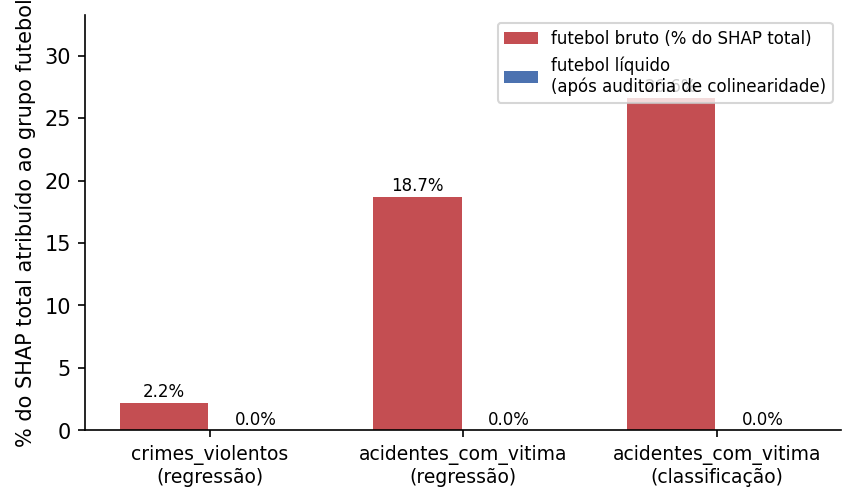
\includegraphics[width=.9\linewidth]{figuras/futebol_liquido.png}
\caption{Participação do grupo de atributos de futebol no SHAP total,
bruta e líquida de artefato de colinearidade com calendário, nos três
modelos de produção}
\label{fig:futebol}
\end{figure}

\begin{figure}[ht]
\centering
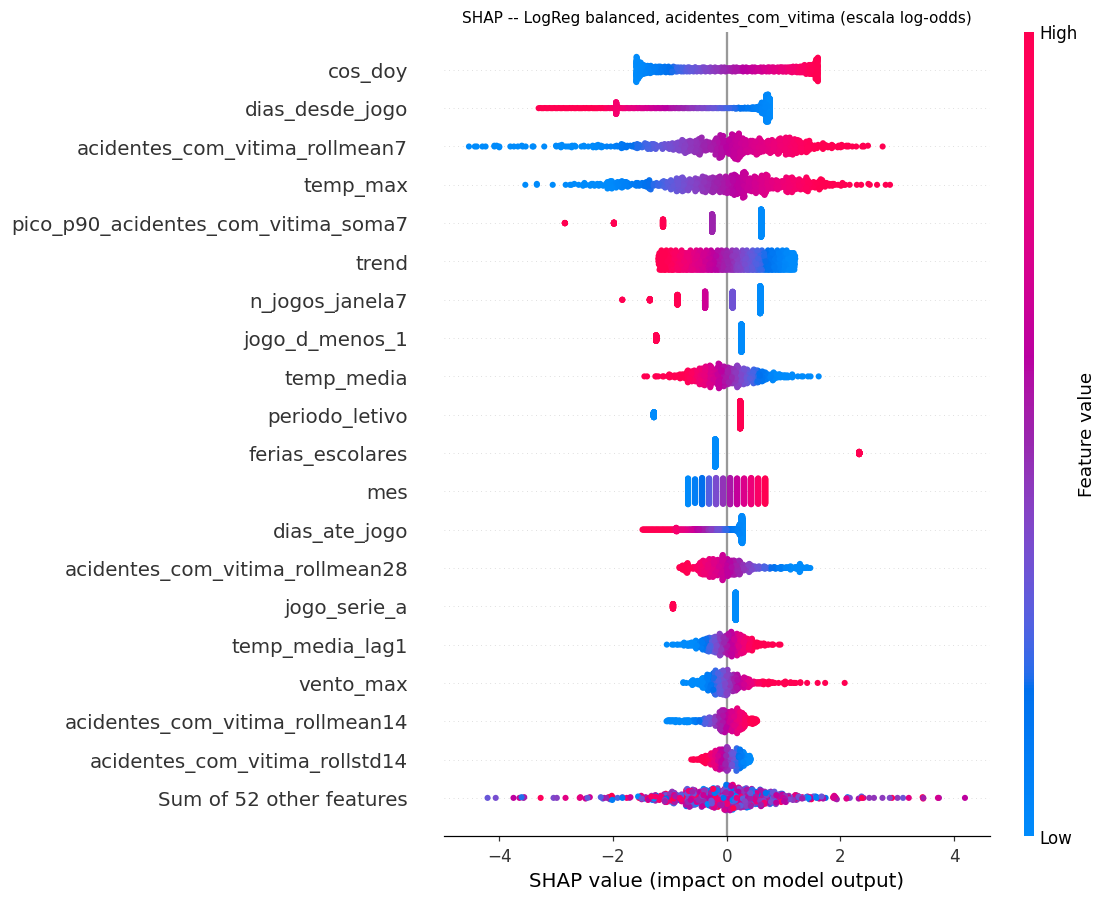
\includegraphics[width=.85\linewidth]{figuras/shap_beeswarm_acidentes.png}
\caption{Valores de SHAP por atributo, Regressão Logística balanceada,
classificação de pico de sinistros com vítima. Atributos de futebol como
\texttt{dias\_desde\_jogo} aparecem com magnitude elevada mas
correlacionam quase perfeitamente com a época do ano, não com o alvo já
dessazonalizado}
\label{fig:beeswarm}
\end{figure}

A conclusão se manteve estável ao substituir os hiperparâmetros de
produção pelos hiperparâmetros rasos usados na validação temporal
(variação bruta de até 5,7 pontos percentuais entre as duas escolhas de
hiperparâmetro, participação líquida sempre $0,0\%$ nos três modelos),
afastando a hipótese de que fosse um artefato da busca de
hiperparâmetros.

\begin{figure}[ht]
\centering
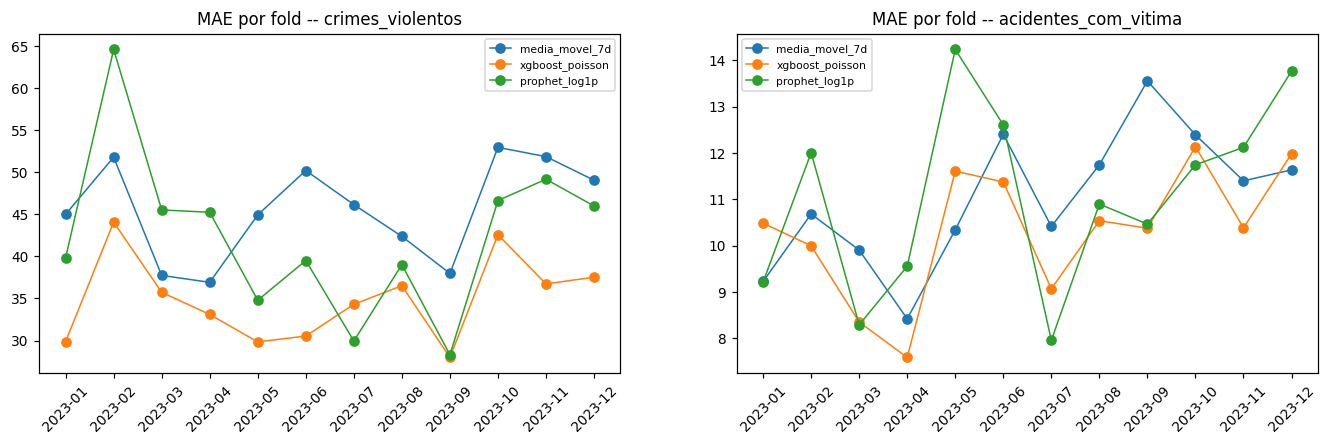
\includegraphics[width=.85\linewidth]{figuras/mae_por_fold.png}
\caption{Erro absoluto médio por \emph{fold} mensal de teste, principais
modelos de regressão}
\label{fig:mae_fold}
\end{figure}

\begin{figure}[ht]
\centering
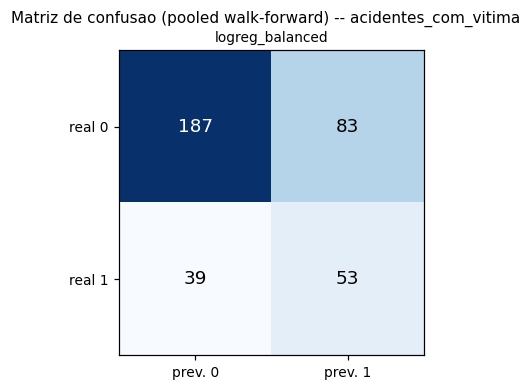
\includegraphics[width=.7\linewidth]{figuras/matriz_confusao_acidentes.png}
\caption{Matriz de confusão \emph{pooled}, Regressão Logística
balanceada, sinistros com vítima}
\label{fig:confusao}
\end{figure}

\subsection{Análise de cenários}

Simulações de cenário construídas sobre dias reais do conjunto de dados
(Tabela~\ref{tab:cenarios}) -- domingo com jogo comum, domingo com
clássico, quarta-feira com jogo noturno, e domingo com clássico sob
chuva -- estimaram, para sinistros com vítima, as probabilidades de pico
listadas abaixo, contra $0,203$ e $0,177$ em dias de referência sem jogo
pareados por dia da semana e época do ano.

\begin{table}[ht]
\centering
\caption{Predições por cenário (dias reais como âncora)}
\label{tab:cenarios}
\small
\begin{tabular}{@{}lrrr@{}}
\toprule
\textbf{Cenário} & \textbf{Crimes viol.} & \textbf{Sinistros c/ vítima} & \textbf{$P$(pico)} \\
\midrule
A: domingo + jogo comum      & $508,3$ & $79,4$ & $0,855$ \\
B: domingo + clássico        & $589,4$ & $85,6$ & $0,539$ \\
C: quarta + noturno          & $510,7$ & $86,4$ & $0,627$ \\
D: domingo + clássico + chuva & $576,1$ & $85,7$ & $0,465$ \\
Baseline domingo (sem jogo)  & $491,9$ & $79,3$ & $0,203$ \\
Baseline quarta (sem jogo)   & $544,0$ & $80,9$ & $0,177$ \\
\bottomrule
\end{tabular}
\end{table}

Chama atenção que o cenário de maior risco previsto para sinistros com
vítima tenha sido o de jogo comum (A), não o clássico (B): a decomposição
aditiva dos valores de SHAP entre cada cenário e sua referência
(Tabela~\ref{tab:decomposicao}) mostrou que essa diferença é explicada
majoritariamente por características incidentais do dia real usado como
âncora (histórico recente, clima), não pelo tipo de jogo -- uma
ilustração concreta de por que comparar cenários sem decompor a
contribuição de cada grupo de atributos pode induzir a uma leitura
causal equivocada.

\begin{table}[ht]
\centering
\caption{Participação do grupo futebol no delta cenário-vs-baseline (\%
do ``tamanho'' do delta, escala aditiva do modelo)}
\label{tab:decomposicao}
\small
\begin{tabular}{@{}llr@{}}
\toprule
\textbf{Comparação} & \textbf{Alvo/tarefa} & \textbf{\%|futebol|} \\
\midrule
A vs.\ baseline domingo & Crimes violentos (regr.)    & $0,3$  \\
A vs.\ baseline domingo & Sinistros c/ vítima (regr.) & $2,7$  \\
B vs.\ baseline domingo & Crimes violentos (regr.)    & $19,6$ \\
B vs.\ baseline domingo & Sinistros c/ vítima (regr.) & $4,1$  \\
C vs.\ baseline quarta  & Crimes violentos (regr.)    & $26,6$ \\
C vs.\ baseline quarta  & Sinistros c/ vítima (regr.) & $9,4$  \\
D vs.\ B (só chuva muda) & Sinistros c/ vítima (regr.) & $0,2$  \\
B vs.\ baseline domingo & Sinistros c/ vítima (class.) & $32,7$ \\
\bottomrule
\end{tabular}
\end{table}

Na maioria das comparações, o grupo futebol responde por uma fração
pequena do delta total -- reforçando o nulo das seções anteriores. A
exceção parcial é a classificação de sinistros com vítima (cenário B),
onde o futebol responde por $\sim$33\% do delta desse par específico de
dias -- ainda minoritário, e não a mesma quantidade que a participação
líquida global do grupo (que a auditoria da Seção
\ref{sec:interpretabilidade} fixou em $0,0\%$): um mede o delta de 2 dias
reais específicos, o outro a média sobre todos os dias.

\section{Discussão}

O contraste entre esta investigação e a literatura de referência
\cite{kurland2014,ristea2018,ristea2020} é informativo por si só. Esses
trabalhos, operando em janelas espaciais de poucos quilômetros e horas em
torno de um único estádio, encontraram associações mensuráveis entre dia
de jogo e criminalidade local. Aqui, na escala da cidade inteira e do dia
inteiro, a associação bruta observada -- em alguns desfechos, de
magnitude comparável à relatada na literatura internacional --
desapareceu sistematicamente após o controle por calendário, e nenhum
dos sete métodos independentes aplicados (regressão ajustada, correlação
parcial, defasagem distribuída, \emph{Difference-in-Differences},
pareamento por escore de propensão com IPTW, adaptação de séries
temporais interrompidas, e auditoria de colinearidade em SHAP) encontrou
evidência robusta em contrário. Isso não contradiz necessariamente a
literatura internacional: é compatível com a hipótese, levantada pelos
próprios autores de referência sob a forma do problema da unidade de
área modificável (MAUP), de que um efeito real e espacialmente
concentrado no entorno imediato de um estádio pode se diluir até
desaparecer quando agregado à cidade inteira. O caso do Morumbi, cujo RR
aparente de $2,39$ se revelou artefato de duas datas extremas, de
\emph{pile-up} de geocodificação e de composição majoritária de furto
simples, é uma demonstração concreta desse mecanismo dentro do próprio
estudo -- não uma prova de que o efeito local citado na literatura seja
inexistente, mas uma evidência de que a escala de análise importa tanto
quanto o método estatístico escolhido.

Uma segunda leitura possível é específica do contexto brasileiro: com
três clubes de série A mandando jogos na capital e uma agenda que cobre
quase todo o ano entre campeonatos estadual, nacional e copas, ``dia de
jogo'' em São Paulo é um evento frequente (126 de 730 dias, mais de um
sexto do período) e fortemente concentrado em fins de semana --
justamente o principal fator de confusão identificado. Nesse regime de
alta frequência, o jogo de futebol se aproxima mais de uma característica
rotineira do calendário urbano do que de um evento raro e saliente, o que
pode explicar por que o sinal, se existe, é dominado pelo próprio
calendário antes mesmo de qualquer modelagem. Note-se ainda que a base de
futebol usada não cobre Campeonato Paulista nem Libertadores: dias de
jogo dessas competições entram como ``sem jogo'', o que só pode ter
atenuado qualquer efeito real -- torna o nulo encontrado, se algo,
conservador quanto à direção do viés.

Do ponto de vista preditivo, o desempenho assimétrico entre os dois
alvos merece registro: sinistros com vítima admitiram um classificador
de pico com Recall utilizável, enquanto crimes violentos não. Como o
histórico do próprio desfecho é o grupo de atributos mais importante em
ambos os modelos (Seção \ref{sec:interpretabilidade}), essa assimetria é
mais provavelmente explicada por diferenças na própria dinâmica temporal
de cada série -- sinistros de trânsito parecem ter um padrão sazonal e
semanal mais previsível a partir de seu próprio histórico do que crimes
violentos -- do que por qualquer variável de futebol. Por fim, o fato de
a otimização de hiperparâmetros não ter produzido ganho relevante em
nenhum dos dois alvos reforça essa leitura: com o volume de dados
disponível (730 dias), o fator limitante da previsão parece ser a
quantidade de sinal presente nas variáveis explicativas, não a
capacidade dos algoritmos testados.

\section{Conclusão}

Este trabalho respondeu, com evidência quantitativa, às 12 perguntas que
orientaram a investigação (roteiro original, Seção 23). \textbf{(1)}
Existe associação bruta fraca entre jogos de futebol e violência em
alguns desfechos específicos, mas essa associação não sobrevive ao
controle por calendário em nenhuma das sete abordagens metodológicas
aplicadas; não há, portanto, evidência de causalidade. \textbf{(2)} O
mesmo vale para sinistros de trânsito; sinistros fatais é o resíduo mais
próximo de significância de todo o projeto (RR$=1,146$, $p=0,063$, não
robusto). \textbf{(3)} Clássicos não apresentam risco maior que jogos
comuns nos dois alvos principais, uma vez descontado o artefato de
colinearidade com calendário identificado no SHAP. \textbf{(4)} Jogos
noturnos idem, para os dois alvos principais. \textbf{(5)} A influência
do público não pôde ser testada, por ausência dessa variável na base
disponível. \textbf{(6)} Não foi identificado um período de maior risco
antes, durante ou depois do jogo: nenhuma das 30 defasagens testadas
(D$-2$ a D$+2$) foi significativa após correção de múltiplas comparações.
\textbf{(7)} As variáveis que de fato explicam os picos de crimes
violentos e de sinistros de trânsito são o histórico do próprio
desfecho, o calendário e o clima -- o grupo de atributos de futebol,
uma vez auditado quanto à colinearidade, explica $0,0\%$ da previsão nos
três modelos avaliados. \textbf{(8)} O melhor modelo de regressão foi um
XGBoost com função de perda de Poisson, para os dois alvos; o melhor
classificador de pico foi uma Regressão Logística balanceada, mas apenas
para sinistros com vítima -- para crimes violentos, nenhum classificador
testado atingiu um ponto de operação útil. \textbf{(9)} O Recall para
identificação de picos variou de $0,576$ a $0,674$ (sinistros com
vítima, conforme o hiperparâmetro); nenhum ponto de operação útil para
crimes violentos. \textbf{(10)} A previsão com um dia de antecedência
mostrou-se possível e validada fora da amostra por validação temporal
\emph{walk-forward}; horizontes de previsão maiores que um dia não foram
testados neste trabalho. \textbf{(11)} A margem de erro foi de $34,8$
crimes violentos por dia (MAPE $7,1\%$, $R^2=0,48$) e $10,3$ sinistros
com vítima por dia (MAPE $12,7\%$, $R^2=0,28$), \emph{pooled}
\emph{walk-forward} sobre $\sim$360 dias de teste. \textbf{(12)} As
limitações do estudo são detalhadas na Seção~\ref{sec:limitacoes}. Em
suma, um sistema operacional de alerta de picos de violência e de
sinistros de trânsito para São Paulo deve se apoiar no padrão histórico
do próprio desfecho, no calendário civil e no clima -- não no calendário
de jogos de futebol dos clubes da cidade.

\section{Limitações}
\label{sec:limitacoes}

Este estudo tem limitações relacionadas à qualidade e cobertura dos
dados, a variáveis não observadas e ao desenho de inferência causal.

\textbf{Cobertura de futebol.} A base utilizada cobre apenas Campeonato
Brasileiro (Séries A/B/C) e Copa do Brasil; jogos do Campeonato Paulista
e da Libertadores não estão incluídos e aparecem como ``sem jogo'', o que
tende a atenuar qualquer efeito real e pode inflar o peso do ``efeito
calendário'' encontrado.

\textbf{Público.} A variável de público pagante é integralmente ausente
na base disponível (fonte Kaggle nunca integrada), o que impediu testar
diretamente se o tamanho do público modula o risco -- pergunta 5 do
roteiro original permanece em aberto.

\textbf{Janela temporal.} A janela de sobreposição das três fontes
principais é curta (730 dias), o que limita tanto a robustez da
validação temporal quanto a capacidade do Prophet de capturar
sazonalidade anual.

\textbf{Censura e lacunas de registro.} 2023-12-30/31 (defasagem de
registro administrativo), 2022-01-17 e 2023-08-07 (falha do fluxo de
notificação Infosiga), 27/11/2023 (falha total do INMET) e 25/08 a
11/09/2023 (sensor de precipitação fora do ar) -- todas tratadas como
ausência, nunca como zero.

\textbf{Outlier de registro.} 19/06/2022 tem um pico de furtos compatível
com lançamento retroativo em lote; tratado como dado ausente na
modelagem, com análise de sensibilidade favorável à conclusão
qualitativa (MAE muda de $39,2$ para $43,1$ ao remover o tratamento, sem
mudar a conclusão).

\textbf{Geolocalização.} $\sim$20\% das coordenadas de crime são nulas,
zero ou externas ao município; o bairro (99,6\% preenchido) foi adotado
como unidade primária para análise espacial. O \emph{pile-up} de
geocodificação no Morumbi (investigado na Seção 5.2) é um lembrete de que
análises espaciais de granularidade fina sobre esta fonte exigem cuidado
extra.

\textbf{Causalidade.} A agenda de jogos não tem variação exógena
conhecida (datas são decididas por federações e emissoras de TV, não
sorteadas), o que impede excluir por completo confundidores não
observados -- mudanças pontuais de política de segurança, operações
policiais específicas ou eventos não futebolísticos coincidentes não
podem ser descartados com 730 dias de dados.

\textbf{Classificação de crimes violentos.} Nenhum classificador testado
(Decision Tree, Random Forest, XGBoost, LightGBM, Regressão Logística,
com e sem otimização de hiperparâmetros) atingiu um ponto de operação com
Recall e PR-AUC úteis ao mesmo tempo para esse alvo.

\textbf{Horizonte de previsão.} Todos os modelos foram validados apenas
para o dia corrente (D0, com informação disponível até o dia anterior);
previsão com dois ou mais dias de antecedência não foi avaliada.

\section{Trabalhos Futuros}

Cinco direções decorrem diretamente das limitações identificadas.
\textbf{Primeiro}, a integração de uma fonte de público pagante por
partida (por exemplo, a base Kaggle já identificada mas não baixada)
permitiria testar diretamente a hipótese de que a magnitude da
aglomeração, e não a mera ocorrência do jogo, modula o risco.
\textbf{Segundo}, a inclusão de Campeonato Paulista e Libertadores (via
fonte secundária, como Wikipedia, com o cuidado de marcar a proveniência)
ampliaria a cobertura do calendário de futebol e reduziria a atenuação
identificada. \textbf{Terceiro}, a extensão do horizonte de previsão para
dois ou mais dias de antecedência tornaria o sistema mais útil
operacionalmente do que a previsão apenas para o dia corrente.
\textbf{Quarto}, modelos espaço-temporais que preservem a granularidade
de bairro -- sem incorrer no problema de geocodificação identificado
neste trabalho, por exemplo filtrando ou ponderando por confiabilidade de
coordenada -- poderiam recuperar um eventual efeito local diluído pela
agregação à cidade inteira, no espírito dos trabalhos de referência
internacionais. \textbf{Quinto}, delineamentos com variação mais próxima
da exógena -- por exemplo, mudanças de mando de campo ou realocações de
jogos por motivos alheios ao calendário, ou mesmo suspensões/adiamentos
não planejados -- forneceriam identificação causal mais forte do que a
disponível em dados puramente observacionais.

\begin{thebibliography}{9}

\bibitem{cohen1979} Cohen, L.~E. and Felson, M. (1979) ``Social change and
crime rate trends: a routine activity approach''. \emph{American
Sociological Review}, 44(4), pp.~588--608.

\bibitem{kurland2014} Kurland, J., Johnson, S.~D. and Tilley, N. (2014)
``Offenses around stadiums: a natural experiment on crime attraction and
generation''. \emph{Journal of Research in Crime and Delinquency}, 51(1),
pp.~5--28.

\bibitem{ristea2018} Ristea, A., Kurland, J., Resch, B., Leitner, M. and
Langford, C. (2018) ``Estimating the spatial distribution of crime events
around a football stadium from georeferenced tweets''. \emph{ISPRS
International Journal of Geo-Information}, 7(2), 43.

\bibitem{ristea2020} Ristea, A., Al Boni, M., Resch, B., Gerber, M.~S. and
Leitner, M. (2020) ``Spatial crime distribution and prediction for
sporting events using social media''. \emph{International Journal of
Geographical Information Science}, 34(9), pp.~1708--1739.

\bibitem{austin2011} Austin, P.~C. (2011) ``An introduction to propensity
score methods for reducing the effects of confounding in observational
studies''. \emph{Multivariate Behavioral Research}, 46(3), pp.~399--424.

\bibitem{bh1995} Benjamini, Y. and Hochberg, Y. (1995) ``Controlling the
false discovery rate: a practical and powerful approach to multiple
testing''. \emph{Journal of the Royal Statistical Society, Series B},
57(1), pp.~289--300.

\bibitem{chen2016} Chen, T. and Guestrin, C. (2016) ``XGBoost: a scalable
tree boosting system''. In: \emph{Proceedings of the 22nd ACM SIGKDD
International Conference on Knowledge Discovery and Data Mining},
pp.~785--794.

\bibitem{taylor2018} Taylor, S.~J. and Letham, B. (2018) ``Forecasting at
scale''. \emph{The American Statistician}, 72(1), pp.~37--45.

\bibitem{lundberg2017} Lundberg, S.~M. and Lee, S.-I. (2017) ``A unified
approach to interpreting model predictions''. In: \emph{Advances in
Neural Information Processing Systems 30 (NeurIPS)}, pp.~4765--4774.

\bibitem{soliani2024} Soliani, R.~D., Argoud, A.~R.~T.~T., Santiago, F.,
Lopes, A.~V.~B. and Emekwuru, N. (2024) ``Catastrophic causes of truck
drivers' crashes on Brazilian highways: Mixed method analyses and crash
prediction using machine learning''. \emph{Multimodal Transportation},
3(4), 100173.

\bibitem{dasilva2025} da Silva, J.~P., Rodrigues-Jr, J.~F. and de
Albuquerque, J.~P. (2025) ``On the power of CNNs to detect slums in
Brazil''. \emph{Computers, Environment and Urban Systems}, 121, 102306.

\end{thebibliography}

\end{document}
